
We now present \emph{symbolic pairwise lockset analysis}, a novel method for data race analysis in device drivers.  In Section~\ref{sec:symbolicpairwise} we describe how the approach works in a semi-formal manner, with respect to a simple concurrent programming model.  In Section~\ref{sec:implementation} we explain how we have implemented symbolic pairwise lockset analysis in a practical tool, \whoop, that can be applied directly to driver source code, to check whether pairs of driver entry points can race with one another.

Our experimental evaluation (Section~\ref{evaluation}) demonstrates that the \whoop technique has value as a stand-alone analyzer, and that results from \whoop can be exploited to significantly boost the performance of a more precise symbolic analysis for concurrency, based on context bounding and stratified inlining, offered by the \corral~\cite{lal2012corral} tool; we discuss the latter approach in Section~\ref{corral}.

\subsection{Symbolic Pairwise Lockset Analysis}
\label{sec:symbolicpairwise}

\ADComment{Top level question about this section: is the motivation super-clear?  Is it obvious why we go for the pairwise approach?}

\PDComment{Mention this somewhere (it was in my previous implementation text)? Two-thread reduction is not a new idea, it has been used before in GPU kernel verification~\cite{bardsley2014engineering} and in model checking of cache coherence protocols~\cite{mcmillan1999verification}.}

Our approach considers, for a given driver, every pair of entry points that can potentially execute concurrently.  For each such pair, we use symbolic verification to check whether it is possible for the pair to race in a shared variable. We soundly model the effects of additional entry points by treating the driver shared state abstractly: when an entry point reads from the shared state, a nondeterministic value is returned.  

Symbolic verification of a pair of entry points works by (i) instrumenting each entry point with additional state to record locksets, and (ii) attempting to verify a sequential program that executes the instrumented entry points in sequence and then asserts that the lockset for each shared variable is non-empty.  Verification of the resulting sequential program can be undertaken using any sound method; in practice we employ the Boogie verification engine~\cite{barnett2006boogie}, which requires procedure specifications and loop invariants to be generated, after which verification conditions are generated and discharged to an automated theorem prover.

We now detail the approach in a semi-formal manner, in the context of a simple concurrent programming model.

\medskip\noindent\textbf{Concurrent Programming Model }
%
We consider a simple concurrent programming model in which an unbounded number of threads execute a set of pre-defined \emph{thread templates}.  At any given point of execution a certain number of threads are active, each thread executing a particular template.  In the context of device drivers, a thread template corresponds to a driver entry point, and multiple instances of the same thread template may execute concurrently, just as multiple invocations of a single driver entry point may be concurrent.  Further threads may be launched at any point during execution; in the context of device drivers this corresponds to the OS invoking additional driver entry points.  For ease of presentation only, our model does not feature aggregate data types, pointers or dynamic memory allocation.  These \emph{are} handled by our implementation, and in Section~\ref{sec:implementation} we discuss interesting practical issues arising from the handling of a full-blown language.

A \emph{concurrent program} is described by a finite set of \emph{shared} variables, $\sharedvars$, a finite set of mutexes, $\mutexes$, and a finite set of \emph{thread templates}.  A thread template, $T$, consists of a finite set of procedures, $\procedures{T}$, and a finite set of private variables, $\variables{T}$.  A designated procedure, $\mainforthread{T} \in \procedures{T}$, denotes the starting point for execution of a template by a thread.  A procedure in $\procedures{T}$ is represented by a control flow graph of basic blocks, where each block contains a sequence of statements.  A basic block either has a single successor or a pair of successors.  In the latter case, an \emph{exit condition} over thread-private variables determines, at runtime, the successor to which control should flow on block exit.

The forms of statements are shown in Figure~\ref{fig:statements}, and include designated statements for reading from and writing to shared variables.  In particular, shared variables may not appear in arbitrary expressions.  This restriction simplifies our presentation of lockset instrumentation, below, and a program that does not satisfy this restriction can be trivially pre-processed into one that does via the introduction of additional private temporary variables to record values read from the shared state.  We do not specify the form of expressions, nor the types of variables, assuming a standard set of data types and operations.

\begin{figure}
\begin{tabular}{lp{5.5cm}}
\textbf{Statement Form} & \textbf{Notes} \\
\toprule

$x = e;$ & private assignment, where $x \in \variables{T}$ and $e$ is an expression over $\variables{T}$ \\
\midrule

$x = f(\overline{e});$ & procedure call, where $x \in \variables{T}$, $\overline{e}$ is a sequence of expressions over $\variables{T}$, $f$ is the name of a procedure in $\procedures{T}$ \\
\midrule

$s = e;$ & shared write, where $s \in \sharedvars$ and $e$ is an expression over $\variables{T}$ \\
\midrule

$x = s;$ & shared read,  where $x \in \variables{T}$ and $s \in \sharedvars$ \\
\midrule

$\mutexlock{m};$   & mutex lock, where $m \in \mutexes$ \\
\midrule

$\mutexunlock{m};$ & mutex unlock, where $m \in \mutexes$\\
\bottomrule
\end{tabular}
\caption{Forms of statements in our simple programming model}
\label{fig:statements}
\end{figure}

\medskip\noindent\textbf{Semantics }
%
Let $\ids$ be an infinite set from which dynamic thread ids will be drawn.  The state of a running concurrent program consists of: a valuation of the shared variables, $\sharedvars$; a mapping that associates each mutex in $\mutexes$ with an id from $\ids$, recording which thread currently holds the mutex, or with a special value $\bot \notin \ids$ to indicate that the mutex is not held by any thread; and a list of \emph{threads}.  Each thread consists of an id, drawn from $\ids$, a thread template, $T$, an index indicating the next statement of $T$ to be executed by the thread, and a valuation of the thread private variables, $\variables{T}$.  If multiple threads are instances of the same template $T$, then each thread carries a \emph{separate} valuation of the private variables for this template.

At the start of execution the valuation of shared variables is arbitrary, no mutexes are held (i.e.\ each mutex maps to $\bot$), and the list of threads is empty.

At any point of execution, a new thread may be added to the list of thread states.  This involves selecting an id $i \in \ids$ that has not been previously used during program execution and a thread template $T$, setting the point of execution for the new thread to be the first statement of $\mainforthread{T}$, and choosing an arbitrary valuation for the private variables $\variables{T}$.

We consider a standard interleaving model of concurrency: at any execution point, a thread may execute its current statement, unless that statement has the form $\mutexlock{m}$ and mutex $m$ is already held by some thread.  Executing a statement causes the state of the thread, and the shared state, to be updated in a standard manner.  For example, if a thread following template $T$ executes $s = e$, where $s \in \sharedvars$ and $e$ is an expression over $\variables{T}$, the shared variable valuation is updated so that $s$ has the value determined by evaluating $e$ in the context of the thread's private variable valuation.  The thread's next statement is updated \PDComment{Do you mean execute?} according to the control flow graph of the current procedure.

A thread terminates if it reaches the end of $\mainforthread{T}$; in this case the thread is removed from the list of threads.  Because we are interested in the analysis of device drivers, which are \emph{reactive} concurrent programs, we do not consider the notion of global program termination.

\medskip\noindent\textbf{Lockset Instrumentation }
%
Suppose that $S$ and $T$ are thread templates for a concurrent program, including the possibility that $S$ and $T$ are equal. We wish to check whether it is possible for a thread that is an instance of $S$ to race with a thread that is an instance of $T$, in the presence of arbitrarily many further threads that may execute concurrently.

To achieve this, we first \emph{instrument} a thread template for lockset analysis (see Section~\ref{bg:lockset}).  Given an arbitrary symbol, $i$, we define the instrumentation of a template $T$ with respect to $i$, denoted $\instrument{T}{i}$.  There are two aspects to this instrumentation phase: \emph{renaming} and \emph{lockset instrumentation}.

Renaming is straightforward: every private variable $x \in \variables{T}$ used in $T$ is replaced with a renamed variable $\instrument{x}{i}$ in $\instrument{T}{i}$, and every procedure $f \in \procedures{T}$ is renamed (both at its declaration site and at all call sites) to $\instrument{f}{i}$ in $\instrument{T}{i}$.  The purpose of renaming is to ensure that when we analyze a pair of templates, $S$ and $T$, both templates execute distinct procedures and operate on distinct private data.  Shared variables and mutexes are \emph{not} renamed, because these are shared across templates.

\begin{figure}
\begin{tabular}{ll}
\textbf{Original Statement} & \textbf{Instrumented Statement} \\
\toprule

$s = e;$ & $\hasbeenwritten{i} = \hasbeenwritten{i} \cup \{ s \};$ \\
         & $\lockset{s}{i} = \lockset{s}{i} \cap \currentlockset{i};$ \\
\midrule
         
$x = s;$ & $\hasbeenread{i} = \hasbeenread{i} \cup \{ s \};$ \\
         & $\lockset{s}{i} = \lockset{s}{i} \cap \currentlockset{i};$ \\
         & $\havoc{\instrument{x}{i}};$ \\
\midrule
         
$\mutexlock{m};$   & $\currentlockset{i} = \currentlockset{i} \cup \{ m \};$ \\
\midrule

$\mutexunlock{m};$ & $\currentlockset{i} = \currentlockset{i} \setminus \{ m \};$ \\
\bottomrule
\end{tabular}
\caption{Instrumenting statements for lockset analysis}
\label{fig:instrumentation}
\end{figure}

Initially, lockset instrumentation introduces sets that track: the shared variables that have been read from and written to; the mutexes that have been consistently used to protect each variable; and the mutexes that are currently held by a thread.  To this end, when instrumenting template $T$ with respect to symbol $i$, we add the sets $\hasbeenread{i} \subseteq \powerset{\sharedvars}$ and $\hasbeenwritten{i} \subseteq \powerset{\sharedvars}$ to track the shared variables that have been read from and written to, respectively, by the thread executing $T$. For each shared variable $s \in \sharedvars$ we add a lockset, $\lockset{s}{i}$, to record the mutexes that are consistently held when the thread accesses $s$. Finally, we add a current lockset, $\currentlockset{i} \subseteq \powerset{\mutexes}$, to record the mutexes that are currently held by the thread.

The statements of each procedure in $\instrument{T}{i}$ that manipulate shared variables and mutexes are then instrumented to take account of the above sets.  This transformation is described in Figure~\ref{fig:instrumentation}, where for an expression $e$ we use $\instrument{e}{i}$ to denote $e$ after renaming with respect to $i$.  A shared variable assignment, $s = e$, is instrumented by recording in $\hasbeenwritten{i}$ that $s$ has been written to, and updating the lockset for $s$, $\lockset{s}{i}$, to eliminate any mutexes that are not currently held (i.e.\ those mutexes that are not in $\currentlockset{i}$).  Notice that in the instrumented form, the shared variable $s$ is no longer assigned to.  We discuss the reasons for this when we describe \emph{shared state abstraction} below.  A shared variable read, $x = s$ operates analogously, except for the additional $\havockeyword$ command applied to the receiving private variable $x$; again this relates to shared state abstraction and is discussed below.  Instrumentation of mutex manipulation commands, $\mutexlock{m}$ and $\mutexunlock{m}$, involves updating the current lockset, $\currentlockset{i}$, to add and remove mutex $m$, respectively.

\medskip\noindent\textbf{Shared State Abstraction }
%
Recall that while our aim is to perform race analysis for pairs of threads, we must be sure to account for possible side-effects due to other threads that are running concurrently.  The instrumentation of Figure~\ref{fig:instrumentation} achieves this via \emph{nondeterminism}: when reading from a shared variable $s$, a nondeterministic value is returned.  This is reflected by the use of a $\havockeyword$ command, which sets its argument to an arbitrary value.  Because all shared state accesses are abstracted in this fashion, it is possible to completely dispense with the shared variables after the lockset instrumentation has been performed.  As a result, when instrumenting a shared variable write, the effect of the write is not explicitly modeled.

\medskip\noindent\textbf{Sequentialisation }
%
The pseudocode of Figure~\ref{fig:sequentialization} shows the sequential program that we analyze in order to prove race-freedom for a pair of thread templates $T$ and $U$. Assuming that $T$ and $U$ have been instrumented using distinct symbols $i$ and $j$, yielding $\instrument{T}{i}$ and $\instrument{U}{j}$, the sequential program operates as follows. First, the read, write and current locksets for $\instrument{T}{i}$ and $\instrument{U}{j}$ are initialized to be empty, and for each shared variable $s$, the locksets $\lockset{s}{i}$ and $\lockset{s}{j}$ are initialized to the full set of mutexes, $\mutexes$.  The main procedures of the instrumented thread templates, $\mainforthread{\instrument{T}{i}}$ and $\mainforthread{\instrument{U}{j}}$, are then executed in turn (the order does not matter, due to renaming). Finally, an assertion checks for consistent use of mutexes: if $s$ is written during execution of $\instrument{T}{i}$ and accessed during execution of $\instrument{U}{j}$, or vice-versa, then the locksets $\lockset{s}{i}$ and $\lockset{s}{j}$ must contain at least one common mutex.

\begin{figure}
\begin{tabular}{l}
$\currentlockset{i} = \emptyset;$ $\hasbeenread{i} = \emptyset;$ $\hasbeenwritten{i} = \emptyset;$ \\
$\currentlockset{j} = \emptyset;$ $\hasbeenread{j} = \emptyset;$ $\hasbeenwritten{j} = \emptyset;$ \\
\texttt{for} $s \in \sharedvars$ \texttt{do} $\lockset{s}{i} = \mutexes;$ $\lockset{s}{j} = \mutexes;$ \medskip
\\

$\mainforthread{\instrument{T}{i}}();$ \\
$\mainforthread{\instrument{U}{j}}();$ \medskip\\

\texttt{assert} $\forall s \in \sharedvars \; .$ \\

$\quad s \in \hasbeenwritten{i} \cap (\hasbeenread{j} \cup \hasbeenwritten{j}) \vee s \in \hasbeenwritten{j} \cap (\hasbeenread{i} \cup \hasbeenwritten{i}) \implies$ \\

$\quad\quad \lockset{s}{i} \cap \lockset{s}{j} \neq \emptyset;$ \\

\end{tabular}
\caption{The sequential program to be analyzed in order to prove race-freedom for a pair of thread templates}
\label{fig:sequentialization}
\end{figure}

\medskip\noindent\textbf{Soundness }
%
We sketch an argument that if the program of Figure~\ref{fig:sequentialization} is correct, it is impossible for a thread executing template $T$ to race with a thread executing template $U$, under the assumption that the threads are guaranteed to terminate. Let us assume that the program of Figure~\ref{fig:sequentialization} is correct, and suppose (by way of contradiction) that a thread executing $T$ can in fact race with a thread executing $U$, on some shared variable $s$.  By our hypothesis that the program of Figure~\ref{fig:sequentialization} is correct, and that the threads terminate, the assertion checked at the end of the program guarantees at least one mutex, say $m$, belongs to both $\lockset{s}{i}$ and $\lockset{s}{j}$.  By the definition of a lockset (and according to the manner in which shared accesses are instrumented in Figure~\ref{fig:instrumentation}), this means that $m$ is held during every access to $s$ by both $\instrument{T}{i}$ and $\instrument{U}{j}$. As a result, $m$ must be unlocked and locked between the two accesses, which contradicts that the pair of accesses is racing.

We require the threads to terminate because in the presence of non-termination the assertion at the end of Figure~\ref{fig:sequentialization} may not be reached.  The termination analysis problem for device drivers has been widely studied, notably in the context of the Terminator tool~\cite{cook2006termination}. In the remainder of the paper we do not consider termination issues, assuming that the drivers we analyze in our experimental evaluation (see Section~\ref{evaluation}) are indeed terminating.

\subsection{Implementation in \whoop}
\label{sec:implementation}

The simple concurrent programming model discussed in Section~\ref{sec:symbolicpairwise} is deliberately idealistic to describe our symbolic verification technique. In practice, the Linux drivers we analyze are written in the C language, we do not know upfront which are the entry points for a driver, we do not have a named set of locks, and rather than having a given set of named shared variables, we have arbitrary memory accesses via pointers. We now explain how we have taken the conceptual ideas from Section~\ref{sec:symbolicpairwise} and used them to build \whoop, a practical tool for soundly detecting data races in drivers.

\begin{figure*}
\centering
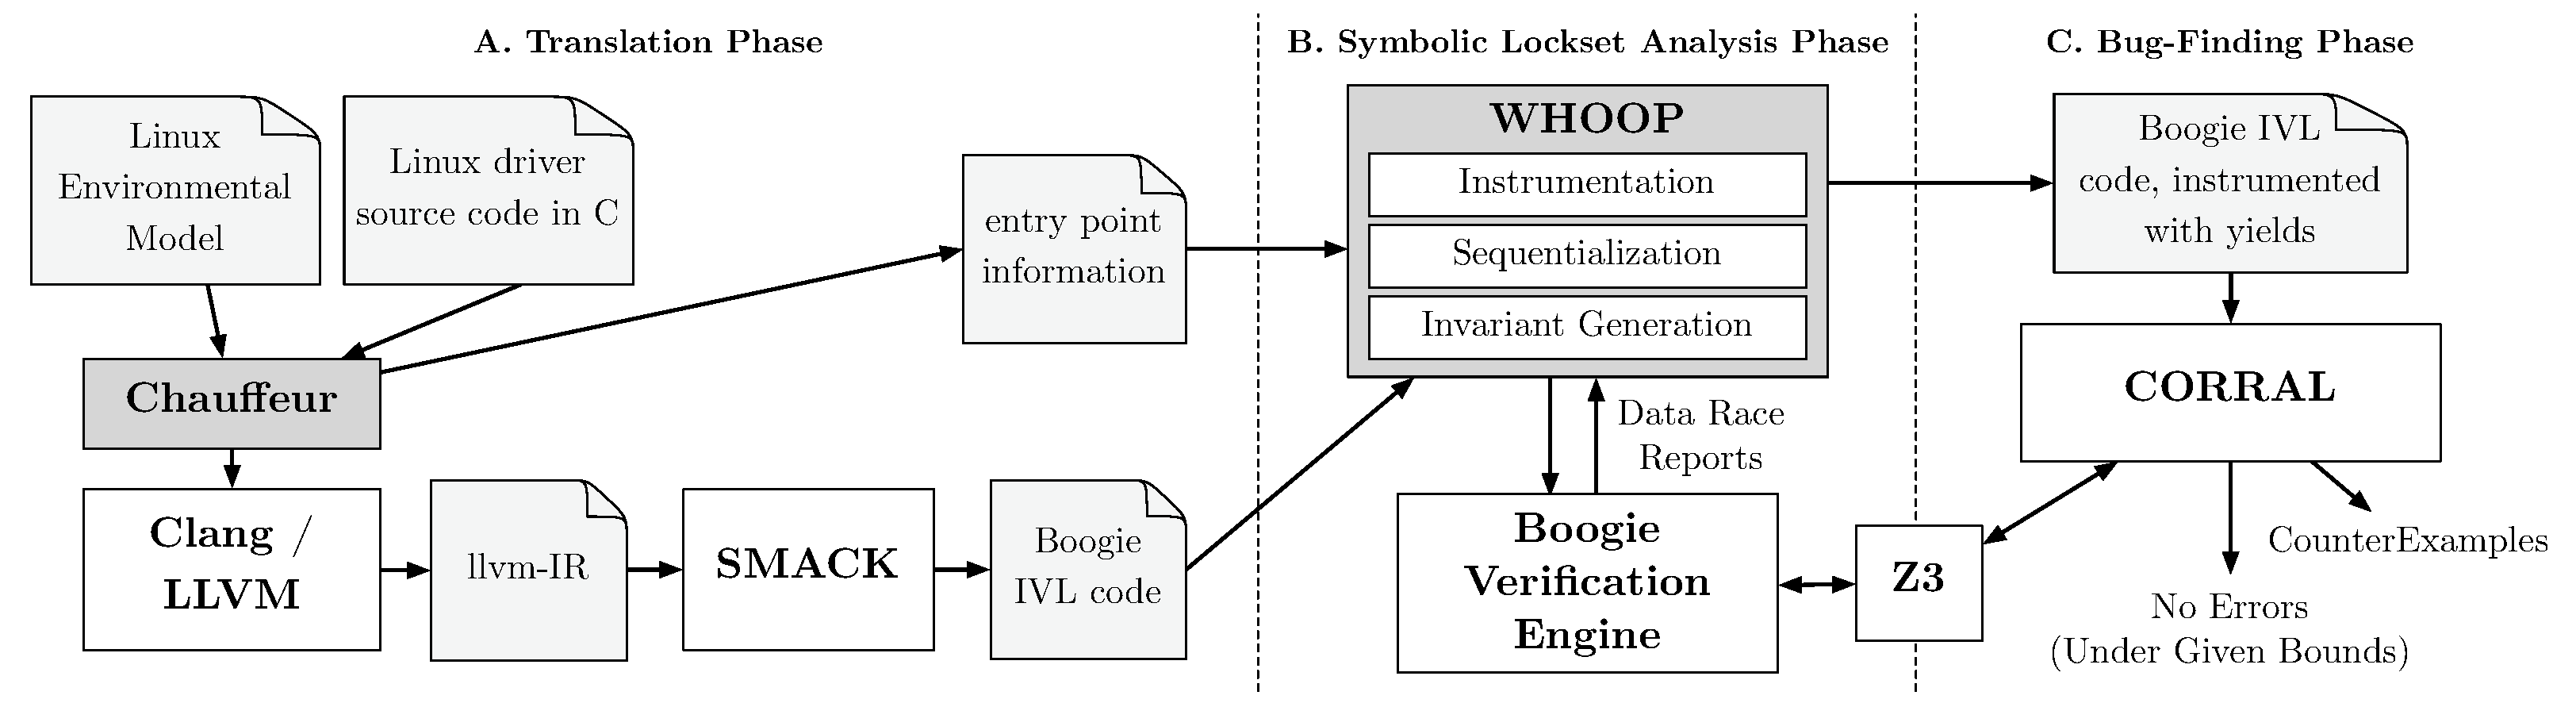
\includegraphics[width=.99\linewidth]{img/whoop.pdf}
\caption{The \whoop architecture, empowered by state-of-the-art compilation (Clang/LLVM and SMACK) and verification (Boogie and \corral) tools}
\label{fig:whoop}
\end{figure*}

\medskip\noindent\textbf{Architecture }
%
Figure~\ref{fig:whoop} depicts the \whoop toolchain. Initially, \whoop accepts a Linux driver written in C, together with an environmental model\footnote{Stub header files that model the Linux kernel APIs.} that is required to ``close'' the driver and allow it to be subsequently analyzed for data races. Both the driver and the Linux model are passed to the translation phase of \whoop (see Figure~\ref{fig:whoop} -- A), which uses three LLVM\footnote{\url{http://llvm.org}}-based tools, Chauffeur\footnote{\url{https://github.com/mc-imperial/chauffeur}}, Clang\footnote{\url{http://clang.llvm.org}} and SMACK\footnote{\url{https://github.com/smackers/smack}}~\cite{rakamaric2014smack}, to translate the original driver into an abstract program written in the Boogie intermediate verification language (IVL)~\cite{deline2005boogiepl}, a simple imperative language with well-defined verification-focused semantics that is used as the input to a number of cutting-edge verifiers (e.g.\ Boogie and \corral).

Next, \whoop instruments and sequentializes the program to perform symbolic pairwise lockset analysis (see Figure~\ref{fig:whoop} -- B and Section~\ref{sec:symbolicpairwise}) using the Boogie verification engine. After the verification phase ends, \whoop can exploit any inferred race-freedom guarantees to accelerate precise race-checking with \corral (see Figure~\ref{fig:whoop} -- C and Section~\ref{corral}).

In this work, we decided to reuse industrial-strength tools, because (i) we did not want to ``reinvent the wheel'' and (ii) these tools are already robust and battle-proven.

\medskip\noindent\textbf{Extracting Entry Point Information }
%
We have developed Chauffeur, a Clang-frontend that performs two important tasks. The first is to traverse (using a Clang visitor pass) the abstract syntax tree (AST) of the original driver and extract all entry point identifier names, together with the identifier names of their corresponding kernel API functions. Linux drivers define entry points in a standard way (see Figure~\ref{fig:entrypoints} for an example of how the generic\_nvram driver defines the entry points for the \texttt{file\_operations} API); Chauffeur identifies these definitions in the AST and outputs the relevant information in an XML file, which is subsequently parsed by \whoop.

\begin{figure}[t]
\begin{lstlisting}
const struct file_operations nvram_fops = {
  .llseek = nvram_llseek,
  .read = read_nvram,
  .write = write_nvram,
  .unlocked_ioctl = nvram_unlocked_ioctl,
};
\end{lstlisting}
\caption{Entry points definitions in the generic\_nvram driver}
\label{fig:entrypoints}
\end{figure}

The second task is to instrument the original driver with a function that calls all entry points, one after the other, passing them parameters of arbitrary value (to over-approximate kernel behavior for soundness). This function effectively acts as the \emph{main} function of the driver and is required so that Clang does not compile away any uncalled entry points (because we closed the environment using stub functions). This simple rewriting does not alter the semantics of the original driver, as \whoop only uses this function to create checker functions and instrument them with calls to entry points (see Figure~\ref{fig:sequentialization} for the pseudocode of such checker function). Chauffeur outputs the rewritten driver in a C file.

\medskip\noindent\textbf{Translation for Verification }
%
The rewritten driver is compiled by Clang to LLVM-IR~\cite{lattner2004llvm}, a low-level assembly-like language in single static assignment (SSA) form. Function calls (e.g.\ for locking and unlocking) are preserved in this translation, which is useful for our lockset instrumentation.

SMACK then translates the driver from LLVM-IR to Boogie IVL, which is the input language of \whoop. An important feature of SMACK is that it leverages the pointer-alias analyses of LLVM to efficiently model the heap manipulation operations of C programs in Boogie IVL. This means that \whoop does not need to directly deal with pointers and alias analysis, a hard problem on its own, allowing us to reuse proven existing techniques and focus instead on verification efforts.

To achieve scalability, SMACK is using a split-memory model instead of a monolithic one that would be difficult for backend verifiers to reason about~\cite{rakamaric2009scalable}. This split memory model is based on \emph{memory regions}, which are maps of integers that model the heap. A benefit of using this model is that memory regions denote disjoint sections of the heap (i.e.\ pointers that cannot alias). We leverage this knowledge inside \whoop to guide and optimize our lockset instrumentation and analysis, and to create a fine-grained granularity of context-switch instrumentation as discussed in Section~\ref{corral}.

In reality, SMACK is unsound ... (e.g.\ integers), but for our work we assume it is sound.

\medskip\noindent\textbf{Identifying Set of All Locks }
%
When the instrumentation phase begins, \whoop performs an inter-procedural static analysis (on the Boogie IVL source code of each entry point) to identify all available locks and rewrite each one (both at declaration and at all access sites) to a unique constant Boogie variable. The reason behind this transformation, is that representing all locks statically, instead of their original SMACK pointer-based representation, helps \whoop perform various internal instrumentation and optimization passes.

Currently, \whoop only supports mutexes and spinlocks from the Linux kernel APIs. However, it is relatively easy to enhance our tool with knowledge of other locking primitives. If \whoop cannot infer a lock, e.g. because it was created dynamically or was indexed from an array of locks, it will exit with a warning. The reason behind this is twofold: (i) it is arguably hard to detect such locks using static analysis; and (ii) we want to advocate the use of good locking practices when developing drivers for the Linux kernel.

\medskip\noindent\textbf{Watchdog Race-Checking Instrumentation }
%
Data race detection is performed by introducing sets containing the locks that are consistently held by each shared variable and sets containing all shared variables that are read and written (see Section~\ref{sec:symbolicpairwise}). Such sets can be typically modeled in Boogie using maps. However, this requires the use of quantifiers to express invariants related to the contents of a set, such as emptiness. To avoid using quantifiers and the associated theorem proving burden, we use instead a \emph{watchdog race-checking instrumentation}, which works as follows:

We introduce a global watchdog variable for each SMACK memory region that is common to both entry points of a pair. This variable is an \emph{unconstrained} constant representing the offset to memory region that should be checked for races. Verification involves proving that two entry points cannot race at the watched offset of every memory region. The arbitrary watched offset implies that every offset of each memory region is race-free. Watchdog race-checking has been used before for verifying GPU kernels~\cite{bardsley2014engineering}.

\medskip\noindent\textbf{Watchdog Summarization }
%
Early on during the development of \whoop, we realized that scalability would be a serious issue. When we tried to apply \whoop on the r8169 ethernet driver ($>$7000 lines of C code) with all functions fully inlined, we run out of memory. One reason was that the C to Boogie translation produced hundreds of thousands of Boogie IVL code, which could not fit in memory. Another reason was that some entry points recursively call helper functions. Inherently, recursion does not work well with inlining. To tackle these issues, we developed \emph{watchdog summarization}, a novel summarization technique that allows us to analyze drivers in a scalable fashion and without destroying precision.

Watchdog summarization uses the Houdini~\cite{flanagan2001houdini} invariant inference algorithm (available inside Boogie) to automatically compute summaries (pre- and post-conditions and loop invariants) from a pool of \emph{candidate} invariants. The reason we need loop invariants is that we over-approximate loops using loop-cutting (also available inside Boogie).

The candidate invariants are based on the aforementioned global watchdog variables that \whoop instruments for watchdog race-checking. The key idea behind watchdog summarization is to automatically generate candidate invariants for each memory region in the granularity of watched accesses. This reduces the false positives from reporting errors if only e.g.\ a field in memory region $\mathit{MR}$ is racing, but the rest of the fields in $\mathit{MR}$ are not racing.

To generate the candidate invariants, \whoop performs an inter-procedural static analysis on the call-graph (in Boogie IVL code) of each entry point, identifying all possible accesses to shared memory locations. To be sound, if \whoop cannot infer information for a specific access, it generates a coarse-grained candidate for the corresponding memory region.

\medskip\noindent\textbf{Verification and Error Reporting }
%
Finally, the instrumented and summarized abstract program is send to the Boogie verification engine, which generates verification conditions~\cite{barnett2005weakest} and discharges them to the Z3~\cite{de2008z3} theorem prover. Successful verification implies that the original program is free of data races, while an error denotes a \emph{potential} data race and is reported to the user. To improve usability, \whoop has a built-in error reporter that matches counterexamples to source code. The following is an example of a reported error:

\begin{lstlisting}
foo.c: error: potential write-write race:
  write by entry point ep1, foo.c:36:2
    shared->resource = 4;
  write by entry point ep2, foo.c:52:2
    shared->resource = 5;
\end{lstlisting}

\medskip\noindent\textbf{Optimizations }
%
To increase precision we enhance \whoop with domain-specific knowledge of how the Linux kernel interacts with its drivers. This is an ongoing manual effort: the more drivers we study, the more domain-specific properties we discover, which we then exploit to make \whoop more precise. In our experience, one of the most effective precision optimizations is to enrich \whoop with information regarding kernel-imposed serialization. The Linux kernel can serialize calls to entry points, thus forcing them to run sequentially with each other. As an example, a large number of networking entry points are mutually serialized with RTNL, a network-specific kernel lock. \whoop exploits this knowledge and does not create pairs for entry points that are serialized.

%Modeling kernel methods is another opportunity to increase precision, but requires Linux kernel expertise. For example, the \texttt{register\_netdev()} function registers a network driver with the kernel. Before this function is called, the kernel is not able to invoke any of the driver's entry points. Modeling this functionality can reduce false positives when race-checking accesses before the driver's registration.

A performance optimization that \whoop uses is to soundly reduce the checked shared variables. If a shared variable $s$ is accessed only by one entry point in a pair, then it is safe to not check $s$ for this pair. This reduces the burden of the SMT solver and speeds up the verification process.

\medskip\noindent\textbf{Assumptions }
%
We assume that the formal parameters of an entry point do not alias, and thus cannot race. This is a potentially unsound feature that can be turned off using a command line option. In our experience so far, though, we have not missed any data races because of this assumption. We also assume that our environmental model and domain-specific knowledge are correct and do not cause any bugs to be missed. Finally, we assume that the external tools we use as part of the \whoop toolchain are sound and bug-free.

\medskip\noindent\textbf{Limitations }
%
\whoop is based on lockset analysis and thus can report false bugs, because a violation of the locking discipline does not always correspond to a real data race (e.g.\ when lockfree synchronization is used instead of locking). \whoop also uses over-approximation (e.g.\ when reading from the shared state) and summarization, which can be sources of false positives. Furthermore, the tool does not currently check for dynamically created locks or for locks that are provided by external libraries, although the later could be addressed by providing a mechanism for users to declare custom locks.

\PDComment{briefly mention interrupts}

Another limitation of \whoop is that it is unable to verify drivers that are designed to be accessed by a single process at a time. This \emph{single-open device}~\cite{corbet2005linux} mode can be enforced by atomically testing (at the beginning of each entry point) a flag that indicates device availability: if the flag is set to true, then the respective entry point executes, else it blocks. Because \whoop performs pair-wise analysis, it over-approximates this flag, and regards a pair of entry points as running concurrently, even if this is not the case. However,~\cite{corbet2005linux} advises against serializing drivers in this way, as it hinders user ingenuity (e.g.\ a user might expect that a device can be accessed concurrently for performance). Because using single-open device mode is considered bad practice, we thus burden the developer with disregarding any related false bug reports.

Statically analyzing system-level software, such as drivers, requires to ``close'' the environment by abstracting away the low level implementation details. In this work, we developed a simple environmental model for the Linux kernel that consists of (nondeterministic) stub functions. A limitation of our model is that it can, and will, ultimately result in decreased precision and, thus, false positives. However, because we currently only focus on finding data races, we can get away with over-approximating a lot of the underlying Linux kernel functionality, without losing too much precision. Enriching our model with domain-specific knowledge to make it more precise is an ongoing manual effort, but requires Linux expertise. We argue that further increasing the precision is orthogonal to the contributions of this paper. Moreover, even if the symbolic lockset analysis results in false positives, \whoop can still use any race-freedom guarantees to significantly speedup a more precise bug-finder, as seen in Sections~\ref{corral} and~\ref{evaluation}.
